\documentclass[11pt]{article}
\usepackage{subcaption}
\usepackage{sectsty}
\usepackage{graphicx}
\usepackage{amsmath} % for 'pmatrix' environment
\usepackage{caption}
\usepackage{subcaption}

% Margins
\topmargin=-0.45in
\evensidemargin=0in
\oddsidemargin=0in
\textwidth=6.5in
\textheight=9.0in
\headsep=0.25in

\title{\textbf{Dokumentation zu:\\DRL-Aufgabenblatt "Markov Decision Processes"}}
\author{Erik Viere, Daniel Hilfer, Domenic Scholz}
\date{\today}

\begin{document}
\maketitle	
\pagebreak

\section*{Aufgabe 3.1}
\subsection*{a)}
Der Algorithmus ist im zugehörigen Jupyter-Notebook dargestellt. Auch die Visualisierungen lassen sich dort finden. Zur Vollständigkeit werden die finalen State Values sowie die finale Policy auch noch einmal in Abbildung  \ref{img:3_1_a} dargestellt. Eine Erklärung der jeweiligen Zeichen ist ebenfalls als Code-Kommentar im Jupyter-Notebook zu finden.\\
Die Konvergenz der State Values tritt in diesem Fall ein, wenn sich kein Wert in der aktuellen Iteration um mehr als $0.001$ geändert hat. Dies dauert $30$ Iterationen für den ersten Durchlauf. Nach diesem wurde die Policy aktualisiert. Der zweite Durchlauf, der bestätigt hat, dass es sich bei der aktualisierten Policy um die beste handelt, brauchte $28$ Iterationen bis zur Konvergenz.

\begin{figure}
    \centering
    \begin{subfigure}[t]{0.32\textwidth}
        \centering
        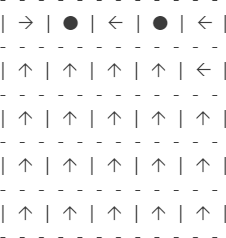
\includegraphics[width=\textwidth]{img/3_1_a1.png}
        \caption{Finale Policy mithilfe bereits konvergierter State Values}
        \label{img:3_1_a1}
    \end{subfigure}
    \hfill
    \begin{subfigure}[t]{0.65\textwidth}
        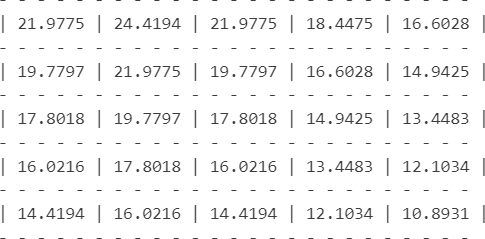
\includegraphics[width=\textwidth]{img/3_1_a2.png}
        \caption{Finale State Values nach Anwendung der optimalen Policy}
        \label{img:3_1_a2}
    \end{subfigure}
    \caption{Ergebnisse des GPI Algorithmus mit vollständer State Value Konvergenz}
    \label{img:3_1_a}
\end{figure}

\subsection*{b)}
Die Implementierung des Algorithmus ist auch für diesen Aufgabenteil im Jupyter-Notebook zu finden. In Abbildung \ref{img:3_1_b} ist eine Auswahl an Iterationen in Form der Policy und der State Values dargestellt. Im beiliegenden Jupyter-Notebook wird jede Iteration visualisiert. Konvergenzkriterium ist hier, so wie in Aufgabenteil a), dass keine State Value des Grids sich um mehr als $0.001$ ändert.\\
Zu sehen ist, dass die State Values etwa $30$ Iterationen bis zur Konvergenz brauchen (genau: $29$), dies gleicht dem Verhalten aus Aufgabenteil a). Hervorzuheben ist jedoch die Konvergenzgeschwindigkeit der Policy. Diese ist bei dem in b) vorgestellten Ansatz schneller, sodass die Policy bereits nach einer State Value Iteration ihren finalen Zustand einnimmt. Dies führt dazu, dass die State Values bereits früh höhere Werte annehmen können und bereits früh die optimalen Entscheidungen getroffen werden jönnen.
Im Vergleich mit der finalen Policy aus Aufgabenteil a) (siehe Abbildung \ref{img:3_1_a}) fällt auf, dass die optimale aus Abbildung \ref{img:3_1_b} leicht von dieser abweicht. Da die State Values jedoch identisch sind (zumindest bis zur 4ten Nachkommastelle) resultiert der Unterschied in den Policies nur aus einer minimalen Abweichung der Werte in den hinteren Nachkommastellen. Der Grund dafür liegt möglicherweise in der Ungenauigkeit der Gleitkommadarstellung und nicht in einem tatsächlichen Qualitätsunterschied der Policies, sodass die Policies als ebenwürdig zu betrachten sind.
Zusammenfassend lässt sich also sagen, dass dieser Ansatz die Lerngeschwindigkeit des Algorithmus maßgeblich steigert.

\begin{figure}
    % Iteration 1
    \begin{subfigure}[t]{0.32\textwidth}
        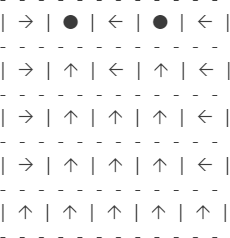
\includegraphics[width=\textwidth]{img/3_1_b_it1_pol.png}
        \caption{Policy after $1$ state value iteration}
        \label{img:3_1_b_1t_pol}
    \end{subfigure}
    \hfill
    \begin{subfigure}[t]{0.65\textwidth}
        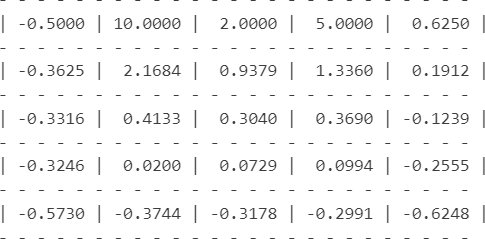
\includegraphics[width=\textwidth]{img/3_1_b_it1_grid.png}
        \caption{State Values after $1$ iteration}
        \label{img:3_1_b_1t_grd}
    \end{subfigure}

    % Iteration 2
    \begin{subfigure}[t]{0.32\textwidth}
        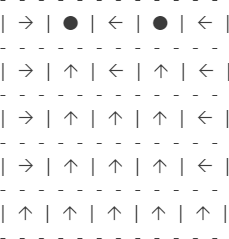
\includegraphics[width=\textwidth]{img/3_1_b_it2_pol.png}
        \caption{Policy after $2$ state value iterations}
        \label{img:3_1_b_2t_pol}
    \end{subfigure}
    \hfill
    \begin{subfigure}[t]{0.65\textwidth}
        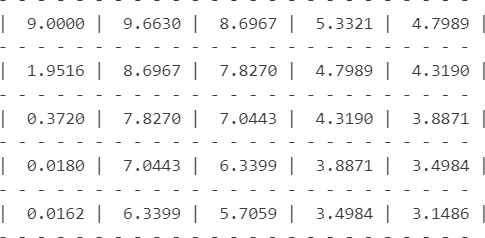
\includegraphics[width=\textwidth]{img/3_1_b_it2_grid.png}
        \caption{State Values after $2$ iterations}
        \label{img:3_1_b_2t_grd}
    \end{subfigure}

    % Final Iteration
    \begin{subfigure}[t]{0.32\textwidth}
        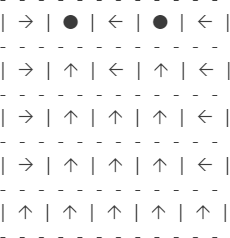
\includegraphics[width=\textwidth]{img/3_1_b_it29_pol.png}
        \caption{Policy after final state value iteration ($29$ iterations)}
        \label{img:3_1_b_final_pol}
    \end{subfigure}
    \hfill
    \begin{subfigure}[t]{0.65\textwidth}
        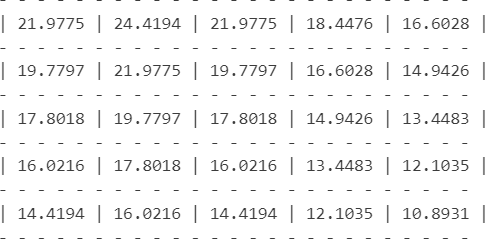
\includegraphics[width=\textwidth]{img/3_1_b_it29_grid.png}
        \caption{State Values after final iteration ($29$ iterations)}
        \label{img:3_1_b_final_grd}
    \end{subfigure}
    \caption{Policy-Improvement mit Update nach jeder State Value Iteration}
    \label{img:3_1_b}
\end{figure}

\subsection*{c)}
Die Unterschiede zwischen der Verwendung der State Values und der Action Values liegen darin, dass bei der Betrachtung der State Values betrachtet wird, welche State Value der resultierende Zustand nach Wahl einer Action hat. Bei der Betrachtung der Action Values wird sich auf die Action Values selbst, in denen jedoch auch die State Values der resultierenden Zustände repräsentiert sind, konzentriert. In beiden Vorgehen ist das Ziel, die optimale Action auszuwählen, nur, dass dazu verschiedene Informationen herangezogen werden.\\
Die Implementierung des GPI Algorithmus mit der Action Value Function ist dem beiliegenden Jupyer-Notebook zu entnehmen. Abbildung \ref{img:3_1_c} zeigt die finale Policy und die resultierenden Action Values.\\
\begin{figure}[t]
    \begin{subfigure}[t]{\textwidth}
        \centering
        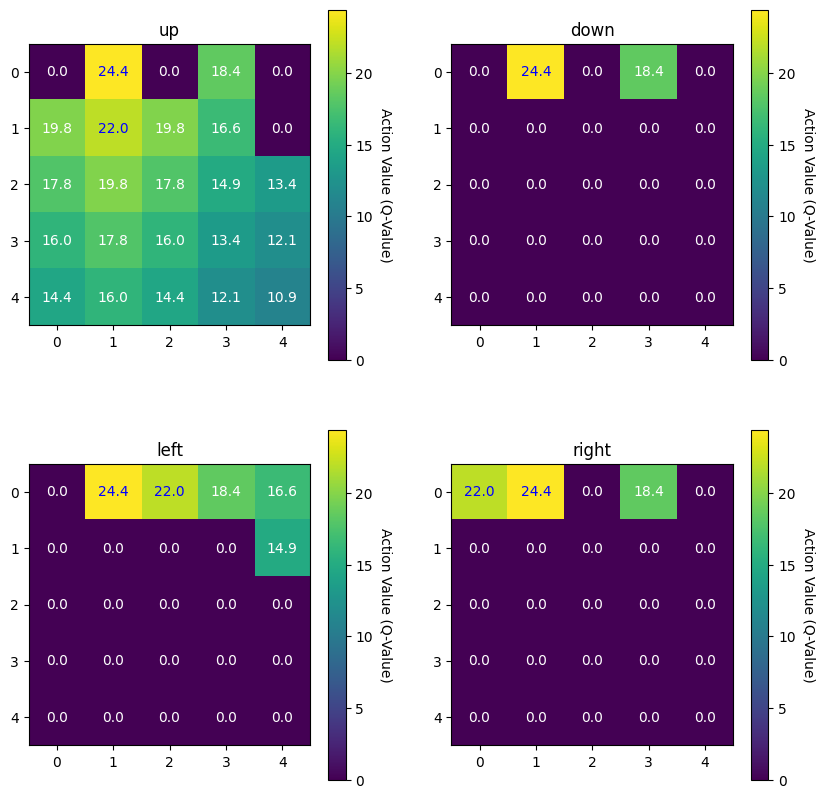
\includegraphics[width=0.95\textwidth]{img/3_1_c.png}
        \caption{Resultierende Action Value Funktionen nach Anwendung von GPI}
        \label{img:3_1_c_heatmap}
    \end{subfigure}
    \begin{subfigure}[t]{\textwidth}
        \centering
        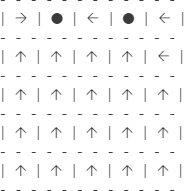
\includegraphics[width=0.33\textwidth]{img/3_1_c2.png}
        \caption{Resultierende Policy nach Anwendung von GPI mit Action Values}
        \label{img:3_1_c_policy}
    \end{subfigure}
    \caption{GPI mit Action Values}
    \label{img:3_1_c}
\end{figure}%
Zu sagen ist, dass sich in diesem konkreten Beispiel die Ansätze nicht drastisch unterscheiden, lediglich der Ansatz, bei der die Policy nach jeder State Value Iteration aktualisiert wird, zeigt eine deutlich schnellere Konvergenzrate. Auch die Action Values benötigen in etwa $30$ Iterationen, um zu konvergieren. Außerdem braucht die Policy, wie bei dem in a) vorgestellten Ansatz, eine Iteration mit konvergierten Action Values, um zur optimalen Policy zu werden.\\
Es kann jedoch sein, dass sich in anderen Beispielen einer der Ansätze eher anbietet. Beispielsweise kann es in modellfreien Umgebungen einfacher sein, die Action Value function zu verwenden, da die beste Action über eine einfache Ermittlung des höchsten Wertes gelingen kann. Die Schätzung der State Values hingegen, die die Action Values implizit verwendet, erfordert eine aufwändigere Interaktion mit der Umgebung, um eine zuverlässige Aussage über die optimale Policy zu ermögichen. Daher kann es in modellfreien Umgebungen schneller zur Konvergenz mithilfe der Action Values kommen, wohingegen eine modellbasierte Umgebung förderlich für die Konvergenzgeschwindigkeit mithilfe der State Values ist.

\section*{Aufgabe 3.2}

\subsection*{a)}
In unserer initialen Policy wird sich zu 80\% in Richtung des Ziels bewegt, also nach rechts oder nach unten.
Eine initiale Policy sollte explorativ sein, damit möglichst viele Wege zum Ziel evaluiert werden.
Außerdem sollte eine initiale Policy das Ziel erreichen können. Wenn für jeden state eine bestimmte Aktion gewählt wird, kann es sein, dass nie ein reward gesammelt wird. Somit haben wir nichts über die Umgebung gelernt.
Eine zufällige Policy kann viele Iterationen benötigen und häufiger schlechte Wege nutzen (z.B. direkt einen Scritt wieder zurück gehen).
Mit der Priorisierung von zielorientierten Wegen sollte schneller eine gute Policy gefunden werden. \\

Die Heatmap aus 3.2 ist in figure \ref{img:heatmap} zu sehen. \\

Da State Values nur den erwarteten return eines states beschreiben, wird nicht näher auf die Rückgabewerte der einzelnen Aktionen eingegangen.
Wenn wir eine optimale Policy finden wollen sind aber gerade die bestimmten Aktionen wichtig mit denen wir einen hohen return bekommen.
Um eine optimale policy zu approximieren brauchen wir also die state action values.
Außerdem können die Monte Carlo Methoden kaum Ergebnisse liefern für Episoden die selten einen reward liefern.
Wie man in figure \ref{img:heatmap} sieht, erhalten wir eigentlich nur nennenswerte Ergebnisse in den states $14$, $13$, $12$ und $11$.
Die restlichen states sind entweder ein Loch oder liefern in zu vielen Fällen keinen reward. Allerdings müssen auch einige states von $0$ - $10$ besucht werden,
jedoch können wir über diese states kaum Aussagen treffen dadurch, dass viele Episoden keinen reward liefern.

\begin{figure}
    \centering
    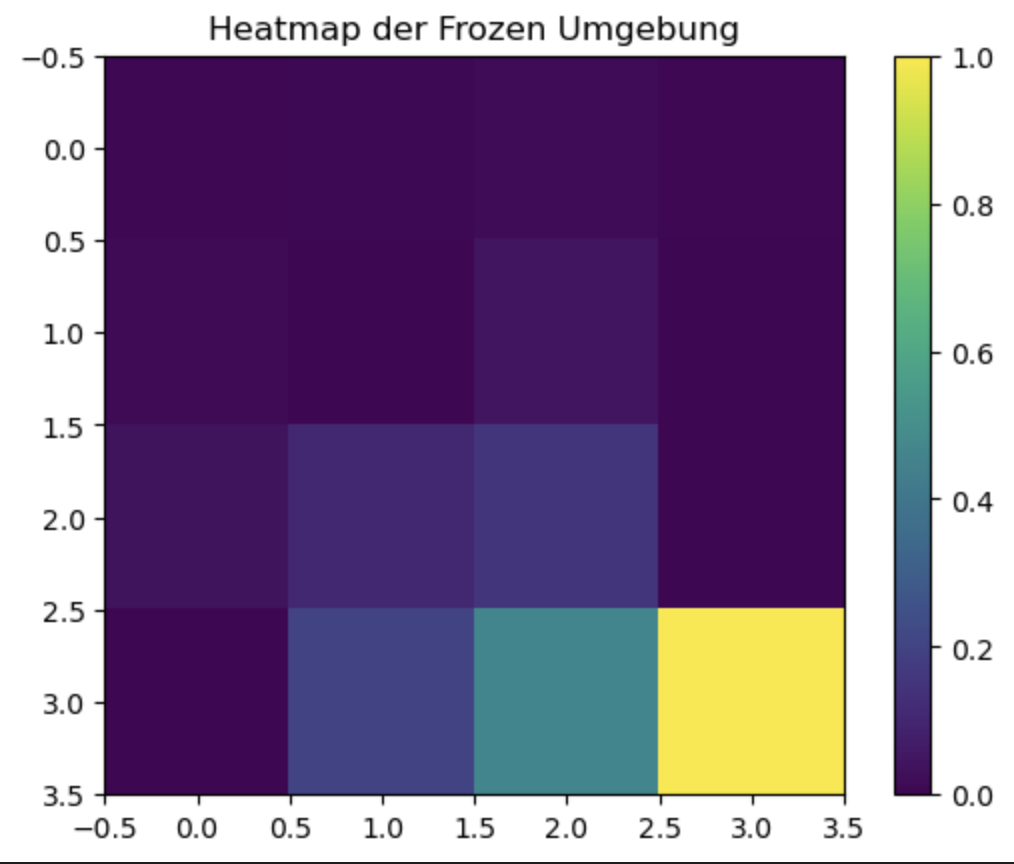
\includegraphics[width=\textwidth]{img/frozen_heatmap.png}
    \caption{Heatmap für die Frozen Umgebung}
    \label{img:heatmap}
\end{figure}

\subsection*{b)}
In figure \ref{img:3_2_b} wird die Summe der returns für mehrere policys dargestellt.
Die beste policy wird danach ausgegeben und ihr gesammelter reward in 5000 Episoden. \\

Für state 3.2 wurden folgende action values berechnet [0.399 0.405 0.408 0.307].
Man sieht, dass die Richtungen links rechts und unten relativ ähnliche returns erwarten.
Das hängt mit der nicht-Deterministischen Umgebung zusammen. Wenn man sich den state als Mensch anguckt, merkt man, dass die logische Entscheidung eigentlich Richtung rechts sein müsste.
Allerdings bedeuted das wählen von Richtung rechts auch nicht zwinged, dass der Spieler sich tatsächlich in diese Richtung bewegt. Tatsächlich kann man mit den Richtungen links rechts und unten
auf jeweils 2 verschiedenen Felder oder dem bisherigen landen, während man mit Richtung oben auf 3 verschiedenen Feldern landen kann und nicht auf dem eigenen Feld bleiben kann.
Dadurch, dass man mit einer Aktion nicht ein bestimmtes, sondern eine Menge von möglichen Zielfeldern auswählt, ist die Aussagekraft eines action values nicht so hoch.




\begin{figure}
    \centering
    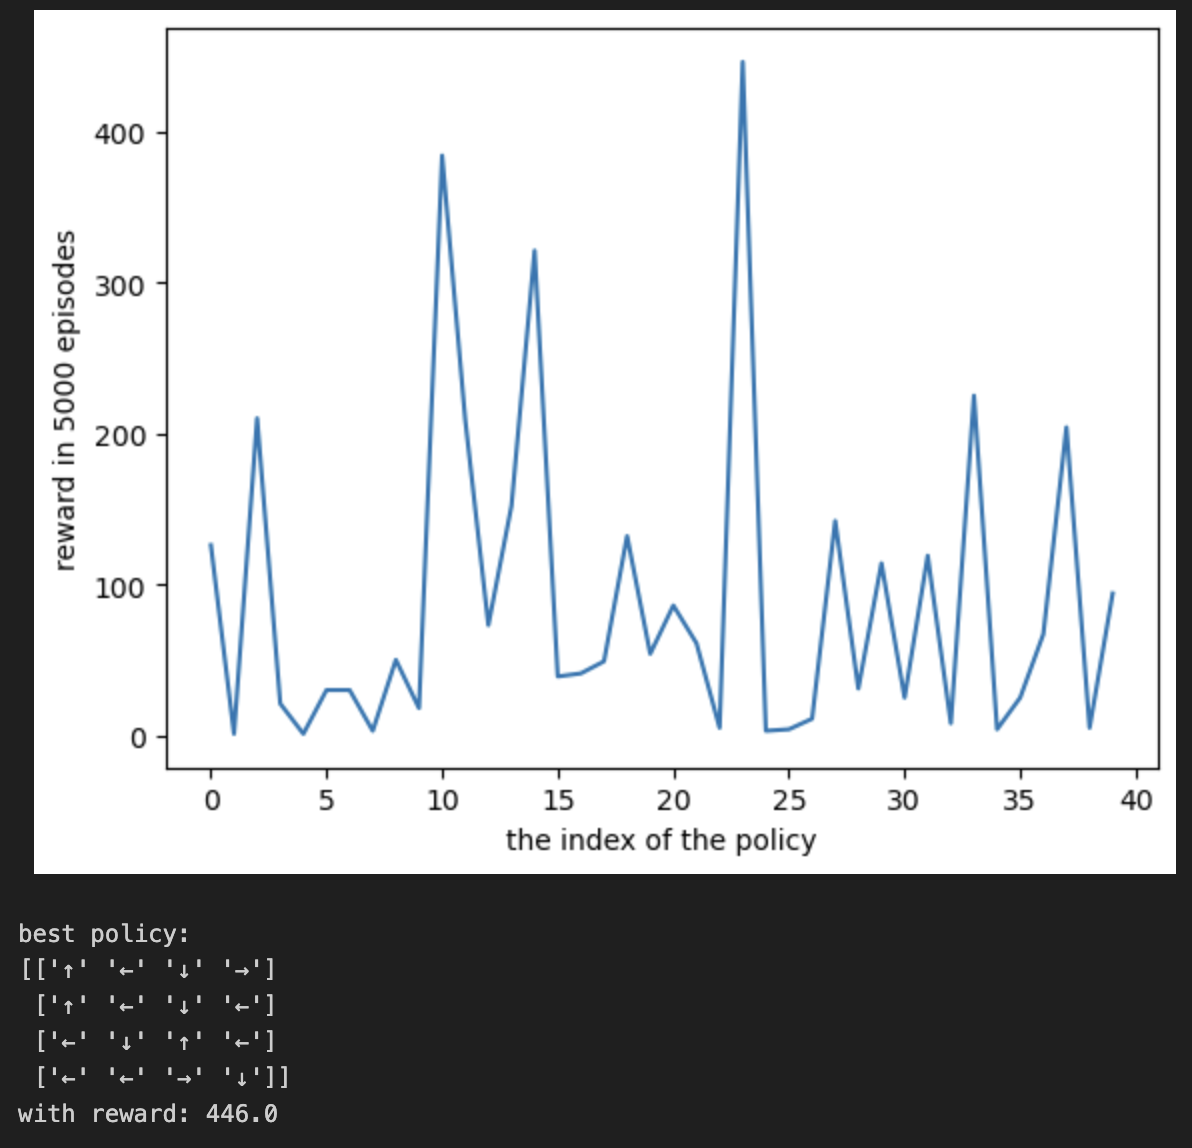
\includegraphics[width=\textwidth]{img/3_2_b.png}
    \caption{Heatmap für die Frozen Umgebung}
    \label{img:3_2_b}
\end{figure}


\end{document}